\documentclass[12pt,a4paper]{article}

%  --  Packages  -- 
\usepackage[utf8]{inputenc}
\usepackage[T1]{fontenc}
\usepackage{lmodern}
\usepackage[margin=2.5cm]{geometry}
\usepackage{setspace}
\usepackage{amsmath,amssymb}
\usepackage{graphicx}
\usepackage[dvipsnames]{xcolor}
\usepackage{booktabs}
\usepackage{natbib}
\usepackage{hyperref}
\usepackage{caption}
\usepackage{subcaption}
\usepackage{enumitem}

\hypersetup{colorlinks=true, linkcolor=NavyBlue, citecolor=NavyBlue, urlcolor=NavyBlue}

\onehalfspacing

%  --  Title  -- 
\title{\textbf{Heterogeneity in the Australian Tax System} \\ \bigskip \large Extended Abstract}
\author{Greg Kaplan\thanks{e61 Institute and University of Chicago.} \and Matthew Maltman\thanks{e61 Institute} \and Matt Nolan\thanks{e61 Institute.}}
\date{May 2026}

\begin{document}
\maketitle

\vfill
% =====================================================================
\begin{abstract}
\noindent Individuals with the same income can pay substantially different effective tax rates, both within a given year and over time. Using the universe of Australian tax returns from 2000 to 2023, we document both dimensions of tax heterogeneity. At the top of the distribution, capital gains treatment is the dominant source of variation. At the bottom, income volatility interacting with the tax-free threshold drives most of the dispersion: individuals moving in and out of work face systematically higher lifetime tax rates than those with stable earnings. Comparing observed outcomes to an income-averaged benchmark, we find that around 80 percent of taxpayers pay more under the current system than they would under smoothing, though changes in tax scales over the period have more than compensated around 20 percent of taxpayers. The progressive schedule provides partial insurance against income shocks, but its cost falls disproportionately on lower-income earners. We decompose the tax gap into contributions from lifecycle progression, idiosyncratic risk, and tax-system changes, showing that the interpretation of horizontal inequity depends on what is treated as ``volatility'' versus foreseeable lifecycle variation.
\end{abstract}

\vfill
\newpage
% =====================================================================
\section{Introduction}

In previous work, \citet{KaplanMaltmanNolan2025} outlined the significant differences in annual average tax rates paid by individuals on the basis of how they earn their income. Differences in deductions, offsets, capital gains treatment, and income splitting generate a wide distribution of effective tax rates at any given income level in any given year. Such differences may reflect real inequities in tax treatment. However, they may also reflect elements of the tax system that are \emph{intended} to reduce inequities over the lifecycle. For instance, the progressive schedule taxes less when income is temporarily low, providing partial insurance against income shocks.

In this paper, we investigate how the tax system treats individuals \emph{over time}, where volatility in earnings may generate different tax rates for individuals with the same long-run income. Under a convex tax schedule, an individual who earns more of their income in a concentrated period will pay more total tax than someone who earns the same amount smoothly. If an individual earns \$100,000 in one year and \$0 the next, they pay more tax than someone earning \$50,000 in each year, despite identical total incomes over the two-year window. This may be perceived as horizontally inequitable, and can be inefficient if individuals change their behaviour to earn income in a smoother way, for instance by strategically timing capital gains realisations when retiring, deferring income, or choosing occupations with less variable earnings at the cost of lower expected income.

We therefore characterise heterogeneity in the Australian tax system along two dimensions: \emph{within-year} differences arising from how income is earned and taxed at a point in time, and \emph{over-time} differences arising from the interaction of income volatility with progressive annual assessment. Both are important, and both have distinct implications for equity and efficiency.

That income volatility generates higher tax under progressive assessment has been understood theoretically since \citet{Vickrey1939}, but its empirical magnitude, and the channels through which it operates, remain poorly characterised for entire populations. At the same time, the progressive schedule provides genuine value as partial insurance against income risk \citep{HeathcoteStorViol2017,Choetal2024}: when income falls, the tax rate falls too, cushioning the blow to after-tax income. The question is whether the insurance benefits justify the costs: both the direct cost of higher lifetime tax rates for volatile earners, and the indirect cost of distortions to income timing and labour supply.

We bring population-level administrative data to bear on these questions. Using PLIDA, we follow the universe of Australian taxpayers over more than two decades, characterising heterogeneity in effective tax rates both within years and across time.

Our key findings are as follows. First, the (prior) capital gains discount does generate significant differences in long-run effective tax rates between high-income individuals, confirming the mechanism that has received the most policy attention. However, we find that there are also \emph{significant} differences in tax rates between relatively lower-income individuals, differences that have received far less attention. These differences at the bottom of the distribution are driven almost entirely by income volatility interacting with the progressive schedule and, in particular, with the tax-free threshold. We quantify the over-time dimension by comparing observed tax outcomes to an ``income-averaged benchmark'' that allocates each individual's total income evenly across years and applies prevailing rates, to identify where volatility translates into systematically higher tax treatment relative to a smooth-income counterfactual.

Second, the progressive system does provide meaningful insurance, dampening after-tax income dispersion relative to pre-tax dispersion. But this insurance is not free. It comes at the cost of systematically higher average tax rates for those with volatile earnings, with the penalty concentrated among lower-income earners for whom even small year-to-year fluctuations push them above and below the tax-free threshold.

Third, changes to the tax system over time have more than compensated around 20 percent of taxpayers for variability in individuals real income. This is due to the counterfactual considered, where horizontal inequity reflects differential tax rates paid on the same income. However, tax scales are often set based on the income distribution at a point in time, naturally generating falling tax rates for the same real income. This implies inequities due to volatile income may be exacerbated or attenuated in real tax systems depending on the lifecycle distribution of income. More broadly, by characterising the types of income shocks that occur, and how lifecycle rather than annual assessment would change tax paid, we are able to estimate the insurance value of progressivity. However, this also reveals a tension between vertical and horizontal equity through time: more redistributive lifetime taxes may impose greater horizontal inequity in the tax paid by similar individuals. This highlights the different normative arguments that bear on the application of annual progressive scales.

Understanding the sources of tax heterogeneity matters for several reasons:

\begin{itemize}
\item \textbf{Horizontal equity.} If individuals with identical lifetime resources pay different lifetime tax purely because of income timing, this may represent a violation of horizontal equity, one of the foundational principles of tax design \citep{Musgrave1990}. However, this may also reflect that horizontal equity comparisons over time are inconsistent in a world with income growth.

\item \textbf{Insurance vs. cost.} The progressive schedule provides partial insurance against income shocks, but the cost of this insurance falls disproportionately on those at the bottom of the distribution. Understanding this trade-off is essential for evaluating whether the current degree of progressivity, and in particular the annual assessment window, represent good policy.

\item \textbf{Behavioural distortions.} If income volatility generates a meaningful tax penalty, individuals have incentives to smooth or time their income, for instance through salary sacrifice, capital gains deferral, income splitting, or adjustments to labour supply. These responses represent a real cost of the current system.

\item \textbf{Lifecycle fairness.} Individuals at the start of their careers face rising tax rates as they move up the progressive schedule, while those approaching retirement benefit from declining rates. Whether this lifecycle pattern represents good design or an unintended penalty on earnings growth depends on whether we view the tax base as annual income or lifetime income.
\end{itemize}

Our paper connects to several strands of the literature.

\paragraph{Progressivity as insurance.} \citet{HeathcoteStorViol2014} develop a framework with partial insurance against wage shocks, finding that approximately 39 percent of permanent shocks pass through to consumption. \citet{HeathcoteStorViol2017} characterise optimal progressivity analytically, showing the trade-off between insurance benefits and distortions to labour supply and skill investment. \citet{Choetal2024} use a BPP approach to estimate the consumption insurance provided by the progressive income tax scale using Australian survey data (the HILDA survey).

\paragraph{Income volatility over the lifecycle.} The literature highlights that there is significant variability in income. \citet{MeghirPistaferri2004} decompose income dynamics into permanent and transitory components with ARCH effects, finding substantial heterogeneity in variance. However, such income variability is also a characteristic of labour earnings. \citet{GuvenOzkanSong2014} use US Social Security Administration data to show that earnings risk is characterised by greater left-skewness in recessions, where large drops become more likely while large gains become less likely. \citet{GuvenEtal2021} document that earnings changes are highly leptokurtic and negatively skewed, with both features varying substantially by age and prior earnings. \citet{Tinetal2025} illustrate similar earnings dynamics in Australia. \citet{StorTelmerYaron2004} show that inequality in both income and consumption increases with age, consistent with highly persistent income shocks accumulating over the lifecycle.

\paragraph{Tax assessment periods and horizontal equity.} \citet{Vickrey1939, Vickrey1947} first identified the horizontal-equity problem created by annual assessment of a progressive tax and proposed cumulative lifetime averaging as the solution. \citet{Weinzierl2011} shows that age-dependent taxes, a step toward lifecycle assessment, capture over 60 percent of the welfare gains from fully dynamic optimal taxation. \citet{FarhiWerning2013} derive optimal dynamic taxes showing that the tax system should provide insurance against persistent shocks while accounting for information revealed over the lifecycle. %\citet{Kaplow2000} challenges whether horizontal equity has independent normative force, arguing it reduces to welfarist concerns -- but even under this view, understanding the sources of differential treatment is essential for evaluating the welfare properties of the system.

% =====================================================================


\section{Data}

We use the \textbf{Personal Longitudinal Integrated Data Asset (PLIDA)}, constructed by the Australian Bureau of Statistics. PLIDA links individual tax returns filed with the Australian Taxation Office (ATO) to Census, health, and other administrative records via a unique person identifier (a statistical linkage key). Our primary analysis uses the tax module, which contains the universe of personal income tax returns filed in Australia from the 1999--2000 financial year to 2022--23.

For each individual--year observation, we observe: total taxable income and its components (wages, business income, investment income, capital gains, government transfers), tax offsets and deductions claimed, and net tax assessed. Demographic information (age, sex, occupation at the 4-digit ANZSCO level, marital status, and number of dependants) is available through linkage to Census and other administrative sources.

Our estimation sample for the core results follows individuals who report positive taxable income in at least 8 of the 11 years from 2012 to 2022. This restriction ensures we observe a meaningful medium-run income trajectory while excluding individuals with minimal labour-force attachment over the period. For robustness and lifecycle analysis, we extend the window back to 2000, giving up to 24 years of panel data.

\paragraph{Income-averaged benchmark.} We compute each individual's long-run average tax rate (ATR) as total tax paid divided by total taxable income over the relevant window. We compare this to a counterfactual ATR computed by allocating each individual's total real income evenly across years and applying the prevailing tax schedule in each year. The difference between observed and benchmark captures the extent to which income volatility, operating through the progressive schedule, translates into higher or lower lifetime tax rates relative to a hypothetical individual with the same total income earned smoothly.

Figure~\ref{fig:context} provides context on the evolution of average tax rates across the income distribution and the concentration of tax payments over our sample period.

\begin{figure}[ht]
\centering
\begin{subfigure}[t]{0.46\textwidth}
\centering
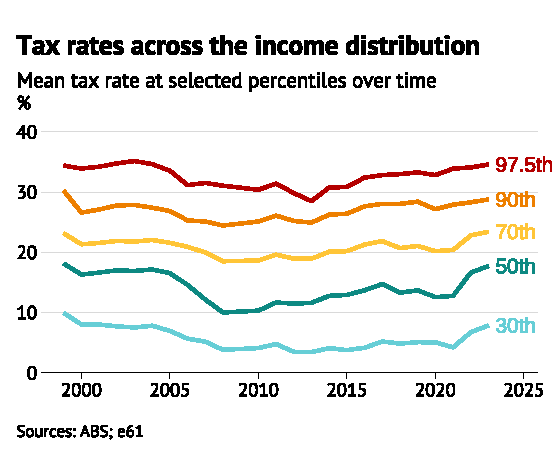
\includegraphics[width=\textwidth]{figures/mean_atr_by_year_percentile.pdf}
\caption{Mean ATR at selected percentiles, 1999--2023.}
\label{fig:atr_time}
\end{subfigure}
\hfill
\begin{subfigure}[t]{0.46\textwidth}
\centering
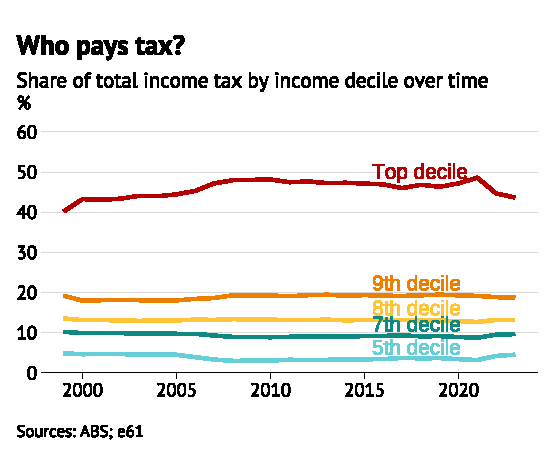
\includegraphics[width=\textwidth]{figures/tax_share_by_decile_time.pdf}
\caption{Share of total income tax by decile, 1999--2023.}
\label{fig:tax_share}
\end{subfigure}
\caption{Context: evolution of tax rates and tax concentration over time.}
\label{fig:context}
\end{figure}

% =====================================================================
\section{Stylised Facts}

We organise our findings around characterising the sources of tax heterogeneity and the role of income volatility.

\subsection{There is substantial heterogeneity in long-run tax rates}

Across individuals with similar total income over 2012--2022, the dispersion in long-run average tax rates is substantial and concentrated at the bottom of the distribution. Figure~\ref{fig:dist_panel} shows both the level and dispersion of effective tax rates across the income distribution. The p10--p90 range exceeds 5 percentage points at the bottom, driven by individuals near the tax-free threshold whose effective rates swing between zero and positive values year to year.

\begin{figure}[ht]
\centering
\begin{subfigure}[t]{0.40\textwidth}
\centering
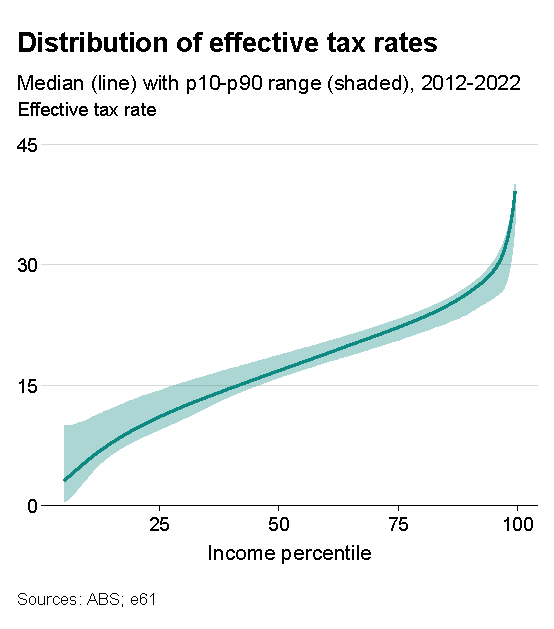
\includegraphics[width=\textwidth]{figures/dist_taxfull_median.pdf}
\caption{Distribution of effective tax rates. Line: median; shaded: p10--p90.}
\label{fig:dist_level}
\end{subfigure}
\hfill
\begin{subfigure}[t]{0.40\textwidth}
\centering
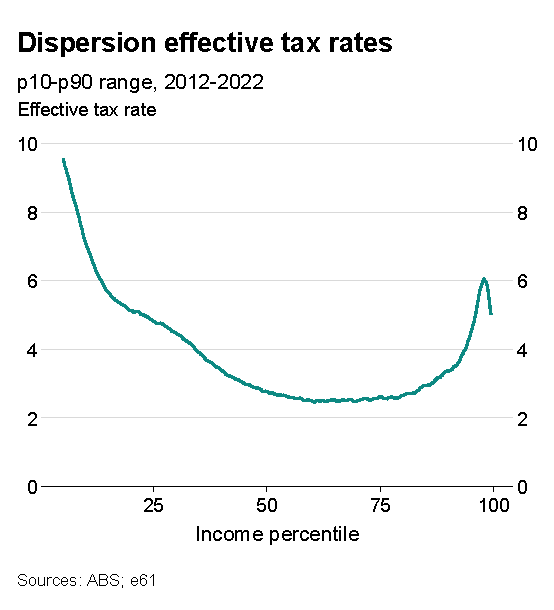
\includegraphics[width=\textwidth]{figures/dist_taxfull_p90p10.pdf}
\caption{Dispersion of effective tax rates (p90--p10 range).}
\label{fig:dist_p9010}
\end{subfigure}
\caption{Distribution and dispersion of long-run effective tax rates, by income percentile, 2012--2022.}
\label{fig:dist_panel}
\end{figure}

\newpage 
\subsection{Income volatility is the dominant driver}

A Shapley-value decomposition of the variance of long-run ATRs into components attributable to (i) income volatility and timing, (ii) Medicare levy interactions, (iii) tax offsets, (iv) select deductions, and (v) capital gains treatment reveals that income volatility accounts for essentially all of the variance at the bottom of the distribution (over 100 percent, offset by negative contributions from other factors) and remains the dominant factor through the 70th percentile. Only at the top of the distribution do capital gains treatment and deductions become quantitatively important (Figure~\ref{fig:decomp}).

\begin{figure}[ht]
\centering
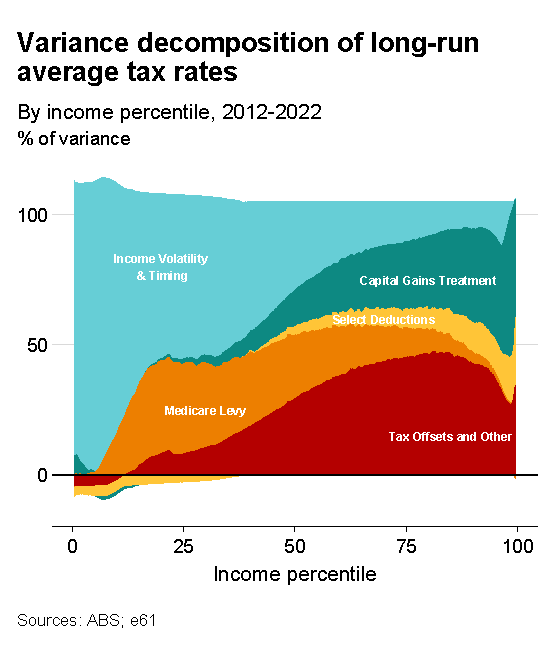
\includegraphics[width=0.60\textwidth]{figures/decomp_stacked.pdf}
\caption{Variance decomposition of long-run average tax rates, by income percentile. Income volatility and timing accounts for essentially all variance at the bottom and remains dominant through the middle of the distribution. Capital gains treatment matters only at the top.}
\label{fig:decomp}
\end{figure}

The mechanism is intuitive. For individuals earning near the tax-free threshold (\$18,200), modest year-to-year variation pushes them above the threshold in some years and below it in others. The convexity of the tax schedule means that the additional tax paid in high-income years exceeds the tax saved in low-income years, generating a systematic upward bias in average tax rates for volatile earners.

\newpage
\section{Income trajectories and horizontal equity}

Interpreting the income-averaging results requires a clear understanding of what is being averaged. Averaging is not a neutral operation. It replaces an observed path of annual income with a counterfactual path, and that counterfactual embodies a judgement about which forms of variation should matter for tax purposes. In a growing economy there are at least four distinct objects that can be averaged away: inflation, aggregate real income growth, predictable lifecycle changes in earnings, and idiosyncratic risk or timing. These objects have different normative interpretations. Treating all of them as ``volatility''
would overstate the extent to which the tax gap reflects risk; treating none of them as volatility would miss the horizontal-equity problem created by annual assessment.

Figure~\ref{fig:averaging-concepts} illustrates the issue with an example.\footnote{We construct a stylised income path with average real income of \$100,000 in 2025 prices. The lifecycle-preserving path is shaped to look more like an empirical wage profile: earnings rise steeply early in the working life and then flatten. The actual path adds mostly small mean-zero residual variation around that lifecycle profile, with a few larger events that can be read as job loss, care responsibilities, or a realised capital gain. The actual and lifecycle-preserving paths therefore have the same lifetime income. We then apply the 1999--00 resident tax scale to each path in Figure~\ref{fig:averaging-concepts}, with thresholds indexed by average economy-wide nominal income growth. This is the tax-system analogue of adjusting for bracket creep: thresholds rise with both prices and average real incomes, so a person whose income remains constant relative to the average taxpayer is not mechanically pushed into higher tax brackets. The benchmark tax rate is therefore the tax rate on the path that is constant relative to average income.} The same observed income path can be compared with several smooth alternatives. A constant-real-income benchmark removes aggregate growth, lifecycle shape, and shocks. A benchmark that is constant relative to average income keeps economy-wide income growth but removes person-specific lifecycle shape and shocks. A lifecycle-preserving benchmark keeps a predictable age or career profile and removes only deviations around that profile. Each comparison answers a different question.

\begin{figure}[htbp]
  \centering
  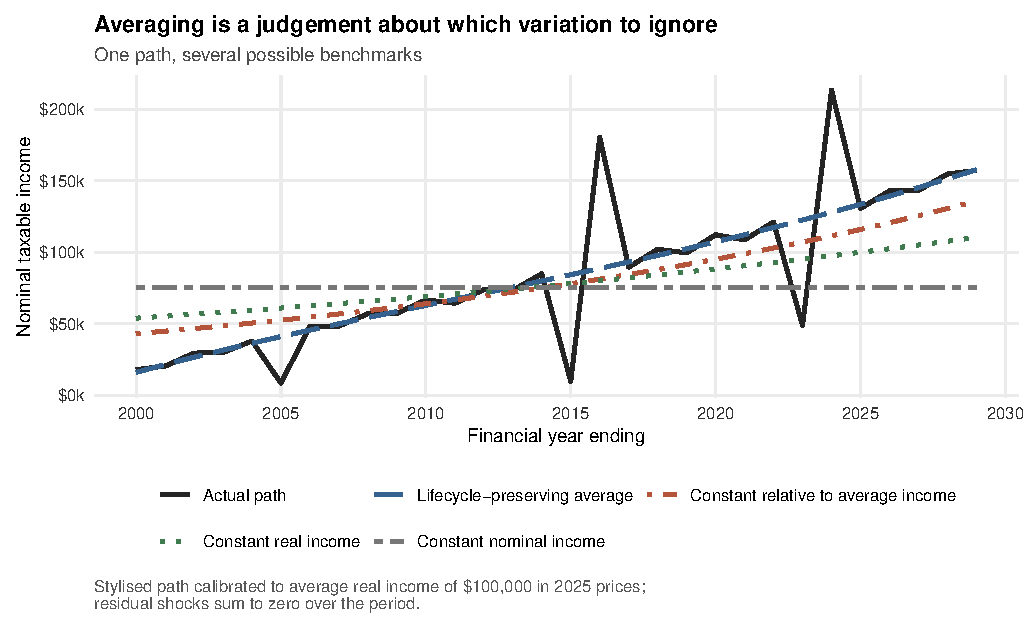
\includegraphics[width=0.94\textwidth]{figures/income_growth_section_averaging_concepts.pdf}
  \caption{Averaging is a judgement about which variation to ignore.}
  \label{fig:averaging-concepts}
\end{figure}

This is where horizontal equity becomes difficult. If horizontal equity means equal tax for equal lifetime real resources, then a constant-real-income benchmark is the natural comparison. Under that view, predictable career growth and involuntary shocks both generate unequal tax treatment because both cause the same lifetime income to arrive in different years. If horizontal equity instead means equal tax for equal lifetime position in the income distribution, then the benchmark should grow with average income. Under that view, a person whose earnings grow with the economy is not becoming richer in the relevant sense. If horizontal equity means equal tax for equal lifecycle opportunity, then the benchmark should preserve expected age-earnings profiles and average only the unpredictable component. Under that view, a young worker's rising earnings are not the same object as an unemployment shock, even if both create convexity costs under annual assessment.



\begin{figure}[htbp]
  \centering
  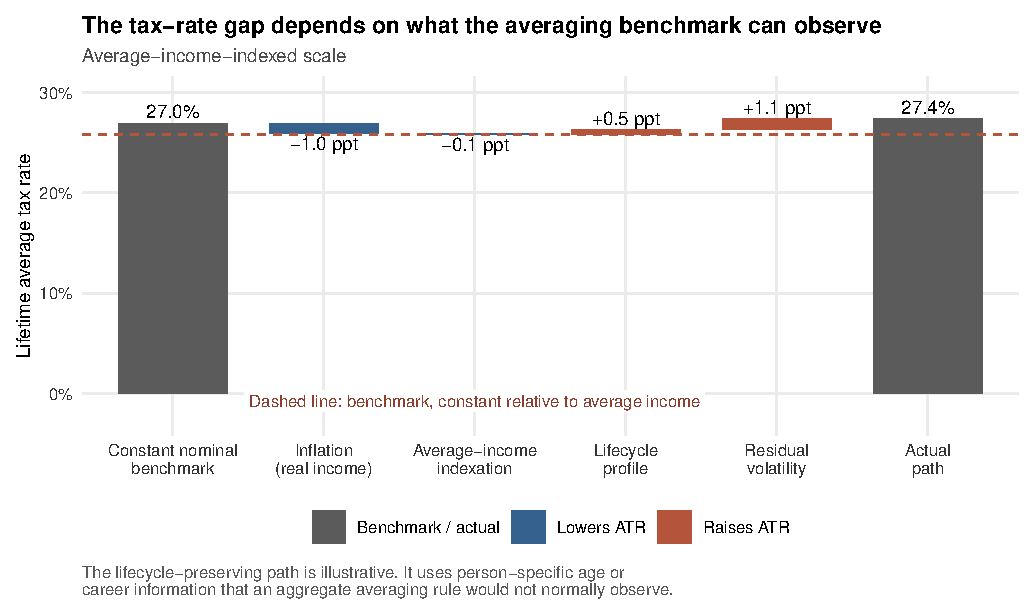
\includegraphics[width=0.94\textwidth]{figures/income_growth_section_averaging_decomposition.pdf}
  \caption{The tax-rate gap depends on what the averaging benchmark can observe.}
  \label{fig:averaging-decomposition}
\end{figure}
\newpage
Figure~\ref{fig:averaging-decomposition} decomposes the tax-rate difference in this example. Here the tax scale rises with average economy-wide income growth each year, thereby adjusting for bracket creep. We can then compare the average tax rate paid over thirty years by a person, depending on how their earnings profile is allocated across years.

The current annual taxation of the lifecycle income path (assuming tax thresholds that adjust for bracket creep) has a lifetime average tax rate of 27.39 percent. If instead the individuals income was \emph{smoothed out} such that they remained at the same percentile in each year (constant-relative-to-average-income benchmark) the tax rate would be a much lower 25.84 percent, or 1.45 percentage points lower.

We can decompose this difference into the contribution of income volatility (where income varied from its lifecycle path) and the contribution of lifecycle effects. In the decomposition, 0.48 percentage points comes from the lifecycle-preserving path: the person has a predictable age or career profile rather than the economy-wide average-growth profile. The remaining 1.08 percentage points comes from residual volatility: the difference between the actual path and the lifecycle-preserving path. This last component is closest to the income-risk or income-timing object that motivates concern about annual assessment.

Real tax systems are unlikely to be able to smooth individuals position in the income distribution, or observe their position on their lifecycle earnings trajectory. As a result, such a system will either average income in nominal terms (splitting dollar amounts through time) or real terms (allocating real income through time). In this example, taxing a constant-nominal-income over time produces a lifetime average tax rate of 26.97 percent. Moving to a constant-real-income benchmark lowers the rate by 1.02 percentage points. The gap between this real system and the distributionally neutral allocation is only 0.11 percentage points. 

This matters for interpreting the PLIDA results. The benchmark used in the empirical figures deflates income by consumer prices, averages it over time, and then re-inflates it to each year. That is closest to a constant real income benchmark: it asks whether a taxpayer paid more than someone with the same real income, even if that income was earned at a different point in time. It is not a pure risk benchmark, nor is it a benchmark that accounts for economic growth increasing everyones position in the income distribution. 

It removes predictable lifecycle growth as well as shocks unless we separately condition on age, sex, family structure,
occupation, or other predictors of normal earnings profiles. But this is precisely the constraint: an administrable averaging rule can use aggregate information such as CPI or average income growth, but it generally cannot know the person's expected lifecycle path. The lifecycle-preserving path in Figure~\ref{fig:averaging-decomposition} is therefore not a proposed operational benchmark. It is an accounting device that shows how much of the measured tax gap would disappear if the benchmark could distinguish predictable lifecycle earnings from residual volatility.

The following empirical task is to separate these components, so that we can ask which part of tax heterogeneity is associated with risk, which part is a penalty on predictable lifecycle patterns, and which part reflects policy (the way changing tax scales map income growth into tax rates).


% =====================================================================
\section{Measuring Sources of Income Volatility and insurance [To be completed]}

The aggregate patterns documented above reflect the combination of several distinct mechanisms generating year-to-year income variation. Understanding these mechanisms matters because they differ in whether the resulting tax heterogeneity represents (i) an unintended cost of annual assessment, (ii) a valuable insurance function, or (iii) an efficient signal for behavioural adjustment.

\begin{enumerate}[label=(\alph*)]
\item \textbf{Lifecycle progression.} Earnings rise steeply in the 20s and 30s as workers accumulate human capital, plateau in the 40s and 50s, and decline toward retirement. This deterministic component moves individuals through progressive tax brackets in a predictable pattern. It is not ``risk'' in any meaningful sense, but rather a foreseeable trajectory, yet it generates differential tax treatment between individuals at different lifecycle stages with the same long-run income.

\item \textbf{Voluntary labour-force transitions.} Childbearing, parental leave, further study, career breaks, and transitions between full-time and part-time work generate large income swings. These are partially within the individual's control and may reflect deliberate lifecycle optimisation.

\item \textbf{Involuntary shocks.} Job loss, firm closure, illness, disability, and relationship breakdown generate income drops outside the individual's control. The progressive schedule provides partial insurance against these shocks, and this is where the insurance interpretation of progressivity is most compelling. But the cost is that individuals who experience more shocks pay more lifetime tax than otherwise-identical individuals.

\item \textbf{Income composition and timing.} Capital gains, business income, and other lumpy income sources are inherently variable. An investment is made given an expected risky rate of return, which ends up being taxed at higher rates due to the progressive tax system. Furthermore, the annual assessment of these sources creates incentives for strategic timing, particularly around retirement, when individuals can realise accumulated gains in low-income years. The (prior) CGT discount partially addressed this for capital income, but no analogous mechanism exists for lumpy wage or business income.
\end{enumerate}

The tax-free threshold plays a disproportionate role in generating tax heterogeneity at the bottom of the distribution. Because the threshold creates a kink in the tax schedule at \$18,200, individuals with average incomes near this level experience large swings in their effective tax rate from year to year. A secondary earner who moves in and out of the labour force, earning \$40,000 in working years and zero in non-working years, pays substantially more lifetime tax than an identical individual earning \$20,000 in every year, despite identical total lifetime earnings.

\subsection{Volatility raises tax rates relative to a smooth-income benchmark}

To quantify how much higher (or lower) tax rates are due to volatility, we compare observed ATRs to the income-averaged benchmark. Under smoothing, most taxpayers would pay less lifetime tax. Figure~\ref{fig:atr_reduction} shows that the reduction in long-run ATRs from smoothing is largest at the bottom of the distribution, exceeding 3 percentage points for individuals with average real income under \$50,000.

\begin{figure}[ht]
\centering
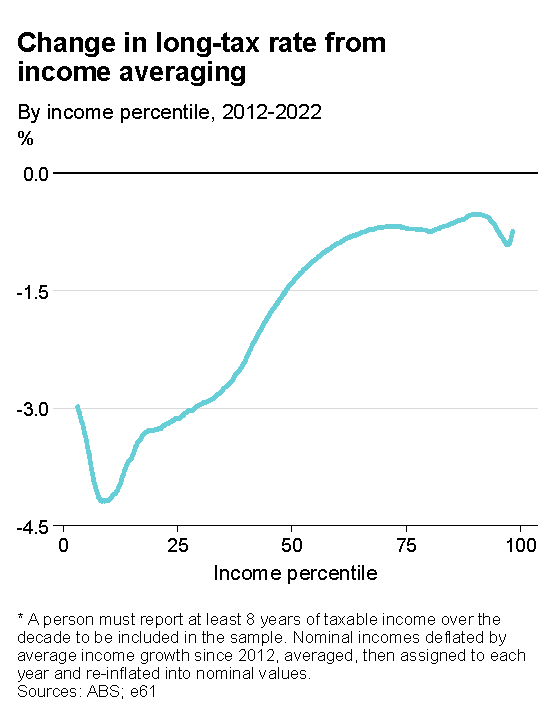
\includegraphics[width=0.55\textwidth]{figures/income_pct_avgincome.pdf}
\caption{Change in long-run tax rate from income averaging, by income percentile, 2012--2022.}
\label{fig:atr_reduction}
\end{figure}

The share of taxpayers who are currently paying \emph{more} than the smooth benchmark exceeds 60 percent across most of the distribution, declining only at the top where volatility sometimes pushes earners \emph{down} brackets (Figure~\ref{fig:betteroff}). Dollar savings are more evenly spread across the distribution due to larger tax bases at the top (Figure~\ref{fig:dollar_share}).

\begin{figure}[ht]
\centering
\begin{subfigure}[t]{0.4\textwidth}
\centering
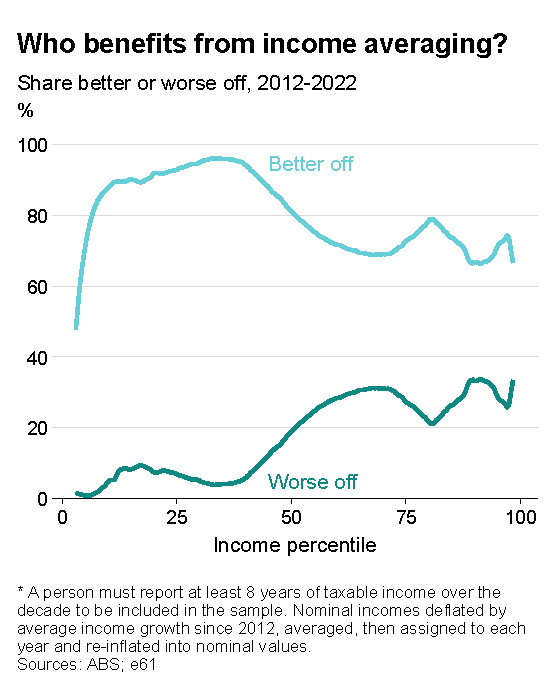
\includegraphics[width=\textwidth]{figures/income_betteroff_avgincome.pdf}
\caption{Who benefits from income averaging?}
\label{fig:betteroff}
\end{subfigure}
\hfill
\begin{subfigure}[t]{0.4\textwidth}
\centering
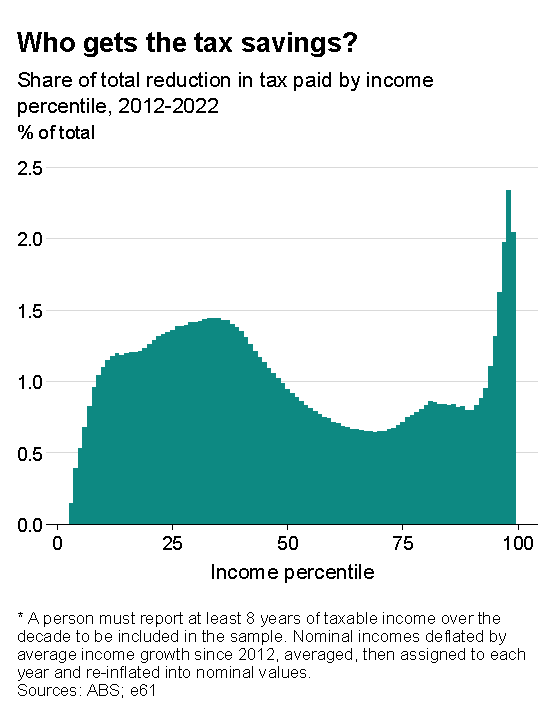
\includegraphics[width=\textwidth]{figures/income_share_avgincome.pdf}
\caption{Who gets the tax savings?}
\label{fig:dollar_share}
\end{subfigure}
\caption{Distribution of benefits from income averaging, 2012--2022.}
\label{fig:who_benefits}
\end{figure}
\newpage
Under a progressive tax system where real tax thresholds remained fixed, any growth or variability in real incomes leads to higher tax rates than a counterfactual where real income is evenly allocated over time. Similarly, a progressive tax system that is only adjusted for bracket creep each year would lead to higher tax rates for those with volatile income or those who earn their income earlier.\footnote{This is an application of Jensen's inequality, where a progressive tax system reflects a convex transformation of incomes.}

However, Figure \ref{fig:betteroff} shows that around 20 percent of individuals would have had a higher average tax liability under averaging than they experienced from the current tax system. This is due to changes in the tax system over this period.

\subsection{The volatility penalty has a clear lifecycle dimension}

The gap between observed and benchmark tax rates varies systematically with age and sex. Young workers experience rising earnings as they progress through their careers, generating a mechanical ``lifecycle creep'' through the progressive schedule. Under the smooth benchmark, some of this tax would be allocated to their lower-earning early years. We find that individuals aged 20--35 see ATR gaps of 1.5--3 percentage points, with the largest effects for women, reflecting greater income disruptions from childbearing and part-time transitions.

A symmetric effect appears at the end of the lifecycle: workers approaching retirement pay more relative to the smooth benchmark because their declining incomes in later years would, under smoothing, pull down tax rates in their peak-earning years.

\begin{figure}[ht]
\centering
\begin{subfigure}[t]{0.46\textwidth}
\centering
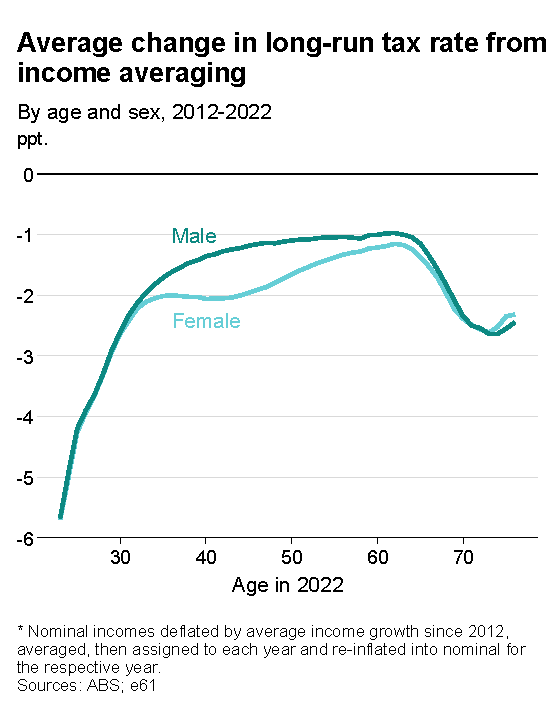
\includegraphics[width=\textwidth]{figures/age_pct_avgincome.pdf}
\caption{Average change in long-run tax rate from income averaging.}
\label{fig:age_pct}
\end{subfigure}
\hfill
\begin{subfigure}[t]{0.46\textwidth}
\centering
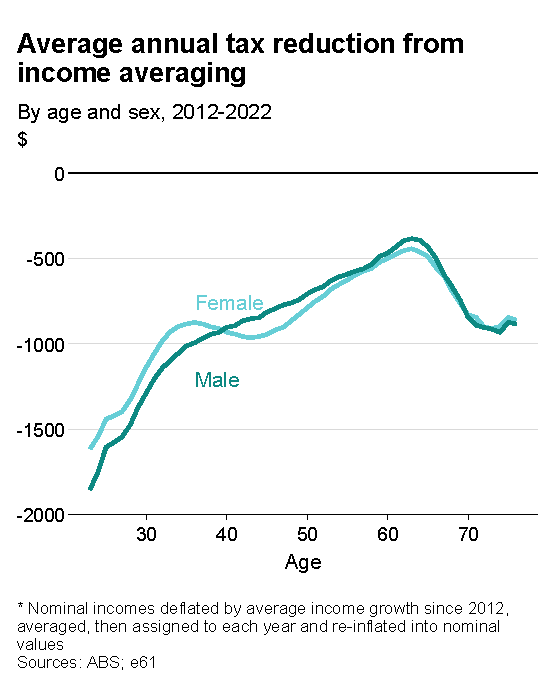
\includegraphics[width=\textwidth]{figures/age_dollar_avgincome.pdf}
\caption{Average annual tax reduction from income averaging.}
\label{fig:age_dollar}
\end{subfigure}
\caption{Lifecycle dimension of the volatility penalty, by age and sex, 2012--2022.}
\label{fig:age_benefit}
\end{figure}

A regression of ATR reduction on demographics confirms this pattern (Appendix Table~\ref{tab:regression}). The largest gains accrue to second earners, unpartnered individuals, and those at either end of the working-age distribution. Women benefit more than men, and the interaction between partnering status and children is quantitatively important.

\newpage
\subsection{Volatility can be separated into clear types}

[TO BE COMPLETED]

\subsection{Distributions under alternative forms of averaging}

[TO BE COMPLETED]

\subsection{The trade-off between lifecycle vertical and horizontal equity}

[TO BE COMPLETED]

% =====================================================================
\section{Discussion and Next Steps}

The findings documented above raise several questions that we intend to pursue in subsequent work. First, we aim to decompose individual income volatility into its component sources (lifecycle progression, voluntary transitions, involuntary shocks, and income composition) and quantify each channel's contribution to observed tax heterogeneity. This will allow us to distinguish the share of heterogeneity that reflects genuine insurance provision from the share that represents an unintended penalty on foreseeable lifecycle patterns.

Second, we will investigate a richer set of definitions of horizontal and vertical equity based on additional counterfactuals. This will allow us to decompose the results \emph{over time} to access the relative role of \emph{income growth} and \emph{income variability}, alongside the related response of the tax system to inflation and income growth. The results in this abstract view horizontal inequity as differential tax rates for individuals with the same real income irrespective of the time period. However, in a world with income growth this would imply rising average tax rates. Instead considering individuals position in the income distribution would allow us to more deeply consider intra-personal and inter-generational distributional issues.

Finally, we plan to investigate the behavioural dimension: whether individuals appear to respond to the volatility penalty by timing income strategically, and whether such responses are concentrated among those with the greatest scope to do so (the self-employed, those with investment income, those approaching retirement). Understanding the extent of income-timing behaviour is important both for assessing the efficiency costs of the current system and for predicting the revenue consequences of alternative assessment designs.

% =====================================================================
% APPENDIX
% =====================================================================
\newpage
\appendix
\section{Regression of ATR Reduction on Demographics}

\begin{table}[ht]
\centering
\caption{Regression of ATR reduction from income averaging on demographic characteristics. Dependent variable: difference between observed and benchmark ATR (positive = paying more under current system). Sample: individuals with 8+ years of positive income, 2012--2022.}
\label{tab:regression}
\small
\begin{tabular}{lcccc}
\toprule
& (1) & (2) & (3) & (4) \\
& No controls & Income FE & No controls & Income FE \\
\midrule
Second earner & 0.048*** & 0.002*** & 0.034*** & $-$0.004*** \\
& (0.000) & (0.000) & (0.000) & (0.000) \\
Unpartnered & 0.060*** & 0.004*** & 0.057*** & 0.003*** \\
& (0.000) & (0.000) & (0.000) & (0.000) \\
1 child & $-$0.037*** & $-$0.023*** & $-$0.033*** & $-$0.017*** \\
& (0.000) & (0.000) & (0.001) & (0.000) \\
2 children & $-$0.028*** & $-$0.014*** & $-$0.039*** & $-$0.019*** \\
& (0.000) & (0.000) & (0.000) & (0.000) \\
3+ children & $-$0.007*** & $-$0.008*** & $-$0.032*** & $-$0.021*** \\
& (0.000) & (0.000) & (0.001) & (0.001) \\
Female & $-$0.021*** & 0.015*** & $-$0.021*** & 0.015*** \\
& (0.000) & (0.000) & (0.000) & (0.000) \\
Age $<$ 30 & 0.095*** & 0.047*** & 0.094*** & 0.046*** \\
& (0.000) & (0.000) & (0.000) & (0.000) \\
Age 30--40 & 0.030*** & 0.023*** & 0.029*** & 0.023*** \\
& (0.000) & (0.000) & (0.000) & (0.000) \\
Age 50--60 & $-$0.008*** & $-$0.014*** & $-$0.009*** & $-$0.014*** \\
& (0.000) & (0.000) & (0.000) & (0.000) \\
Age 70+ & 0.039*** & $-$0.002* & 0.038*** & $-$0.003** \\
& (0.001) & (0.001) & (0.001) & (0.001) \\
\midrule
Partner $\times$ Children & No & No & Yes & Yes \\
Observations & 11,278,162 & 11,278,102 & 11,278,162 & 11,278,102 \\
$R^2$ & 0.037 & 0.147 & 0.038 & 0.147 \\
\bottomrule
\end{tabular}
\begin{minipage}{0.9\textwidth}
\vspace{0.3em}
\footnotesize \textit{Notes:} Standard errors in parentheses. Reference categories: primary earner, no children, male, age 40--50. Columns (2) and (4) include income-percentile fixed effects. *** $p<0.01$, ** $p<0.05$, * $p<0.1$.
\end{minipage}
\end{table}

% =====================================================================
% REFERENCES
% =====================================================================
\newpage
\bibliographystyle{plainnat}
\bibliography{references}

\end{document}
